\chapter{Zarovnávanie sekvencií}

V tejto kapitole si stručne popíšeme čo je to globálne a lokálne zarovnanie a ukážeme základné algoritmy na hľadanie globálneho a lokálneho zarovnania. Tieto algoritmy budeme neskôr modifikované používať pri našom riešení.

\section{Podobnosť sekvencií, sekvenčná homológia a zarovnanie}
V prírode vznikajú nové sekvencie modifikáciou už existujúcich (evolúciou). Preto môžme často spozorovať podobnosť medzi neznámou sekvenciou a sekvenciou o ktorej už niečo vieme. Ak zistíme podobnosti medzi sekvenciami, môžeme preniesť informácie o štruktúre a/alebo funkcii na novú sekvenciu.

Podobné sekvencie, ktoré sa vyvinuli mutáciami so sekvencie v spoločnom predkovi sa nazývajú \textit{homologické} a pod pojmom \textit{hľadanie homológov} rozumieme hľadanie takých podobností, ktoré s veľkou pravdepodobnosťou vznikli práve zdieľanou evolučnou históriou.

%Na prvý pohľad rozhodnutie podobnosti dvoch biologických sekvencií nie je nič iné, ako rozhodnutie podobnosti dvoch textových reťazcov.
%--Tuto vetu tam nechceme--Mnoho metód analýzy biologických sekvencií je preto zakorenená v informatike, kde je už mnoho literatúry týkajúcej sa tejto problematiky.

%Vývoj sekvencií hromadí \textit{inzercie}, \textit{delécie} a \textit{substitúcie}, takže predtým ako môže byť vyhodnotená podobnosť, treba urobiť zarovnanie sekvencií. Preto je zarovnanie sekvencií veľmi dôležité.

Počas evolúcie dvoch homologických sekvencií nastane veľa \textit{inzercií}, \textit{delécií} a \textit{substitúcií}, preto predtým ako môžeme začať porovnávať sekvencie, ich musíme zarovnať tak, aby homologické časti sekvencií boli na rovnakom mieste v zarovnaní.
\cite{durbin, skripta}

\begin{figure}[hbtp]
    \centering
    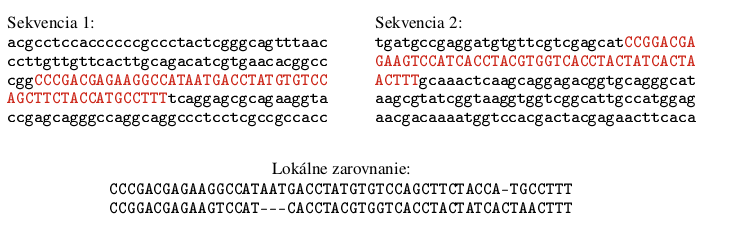
\includegraphics[width=\textwidth]{images/zarovnanie}
    \caption{Lokálne zarovnanie}
    \label{fig:alignment_example}
\end{figure}


\section{Párové zarovnávanie}
Párové zarovnávanie je základná úloha zarovnávania sekvencií, kde sa k sebe zarovnávajú dve sekvencie. V tejto práci sa budeme zaoberať len párovým zarovnávaním.

Kľúčové problémy sú:
\begin{enumerate}
\item Aké typy zarovnávania by sme mali uvažovať
\item Skórovací systém, ktorý použijeme na ohodnotenie zarovnania a trénovanie
\item Algoritmus, ktorý použijeme na hľadanie optimálneho alebo dobrého zarovnania podľa skórovacieho systému
\item Štatistická významnosť zarovnania.
\end{enumerate}

\cite{durbin}

\section{Typy zarovnaní}
Základné typy zarovnaní sú \textit{Globálne zarovnanie} a \textit{Lokálne zarovnanie}.
\begin{df}[Globálne zarovnanie]
Vstupom sú dve sekvencie $X = x_1x_2\dots x_n$ a $Y = y_1y_2\dots y_m$
Výstupom je zarovnanie celých sekvencií $X$ a $Y$ s najvyšším skóre.
\end{df}

\begin{df}[Lokálne zarovnanie]
Vstupom sú dve sekvencie $X = x_1x_2\dots x_n$ a $Y = y_1y_2\dots y_m$
Výstupom je zarovnanie nejakých poreťazcov $x_i\dots x_j$ a $y_k\dots y_l$ sekvencií s najvyšším skóre.
\end{df}
%Pri globálnom zarovnaní je výstupom zarovnanie celých sekvencií s najvyšším skóre.
%Pri lokálnomn zarovnaní je výstupom zarovnanie nejakých poreťazcov sekvencií s najvyšším skóre.
\cite{skripta}

\section{Skórovacie systémy}
Takmer všetky metódy zarovnania hľadajú zarovnanie dvoch reťazcov na základe nejakej \textit{skórovacej schémy}. Skórovacie schémy môžu byť veľmi jednoduché, napr. $+1$ za \textit{zhodu} a $-1$ za \textit{nezhodu}. Hoci ak chceme mať schému, kde biologicky najkorektnjšie zarovnanie má najvyššie skóre, musíme vziať do úvahy, že biologické sekvencie majú evolučnú históriu, 3D štrukturu a mnohé ďalšie vlastnosti obmedzujúce ich evolúciu. Preto skórovací systém vyžaduje starostlivé premyslenie a môže byť veľmi zložitý.
\cite{durbin}

\subsection{Skórovacie matice}
Skoro vždy však chceme rôzne zhody a nezhody skórovať rôzne - nie len všetky zhody $+1$ a nezhody $-1$.
Skóre môže záviseť od toho aké bázy sú v danom stĺpci zarovnania. Na to môžme použiť \textit{skórovaciu maticu}, kde máme definované skóre pre každú dvojicu. Skórovacie matice sa využívajú najmä pri zarovnávaní proteínov, kde niektoré dvojice majú podobné chemické vlastnosti.
\cite{durbin, skripta}

\section[Algoritmy]{Algoritmy na hľadanie zarovnaní}
Máme daný skórovací systém, potrebujeme algoritmus, ktorý nájde optimálne zarovnanie dvoch sekvencií.
Budeme uvažovať zarovnávanie s medzerami. To znamená, že môžeme do sekvencie pridať ľubovoľne veľa medzier, aby sme dosiahli lepšie skóre. Pre 2 sekvencie dĺžky $n$ existuje
$$ {2n \choose n}  = \frac{(2n)!}{(n!)^2} \simeq \frac{2^{2n}}{\sqrt{\pi n}} $$
možných globálnych zarovnaní. Čiže nie je možné v rozumnom čase nimi prejsť.

Algoritmy na hľadanie zarovnaní využívajú \textit{dynamické programovanie}. Algoritmy s dynamickým programovaním garantujú nájdenie optimálneho zarovnania.
Existujú aj heuristické algoritmy, ktoré môžu byť veľmi rýchle, avšak majú určité predpoklady a môže sa stať, že nenájdu najlepšie zarovnanie pre niektoré páry sekvencií.
My sa budeme zaoberať len algoritmami využívajúcimi dynamické programovanie. Pre rôzne typy zarovnaní máme rôzne algoritmy zarovnávania.
\cite{durbin, skripta}

\subsection{Algoritmus pre globálne zarovnanie: Needelman-Wunch}
\label{subsec:global-alignment}
Máme dané 2 sekvencie $X = x_1x_2\dots x_n$ a $Y = y_1y_2\dots y_m$, budeme zarovnávať všetky znaky sekvencie $X$ a všetky znaky sekvencie $Y$.
Definujeme si jednoduchú skórovaciu tabuľku kde $s(x, y)$ bude udávať skóre pre danú dvojicu báz (napr. $+1$ za zhodu, $-1$ za nezhodu) a za nezhodu budeme dávať penaltu $-d$.

%Idea je nasledovná - Nech máme optimálne zarovnanie dĺžky $n$. Zarovnanie dĺžky $n+1$ vieme vyrobiť 3 spôsobmi. Buď pridáme $(x_i,y_j)$, alebo $(x_i,-)$, alebo $(-,y_j)$, kde $i,\ j$ sú indexy prvej nepoužitej bázy v $X$ resp. $Y$. Možnosť s najlepším skore nám dá optimálne zarovnanie dĺžky $n+1$.

\begin{figure}[htp]
    \centering
    \begin{subfigure}[m]{0.5\textwidth}
    \centering
    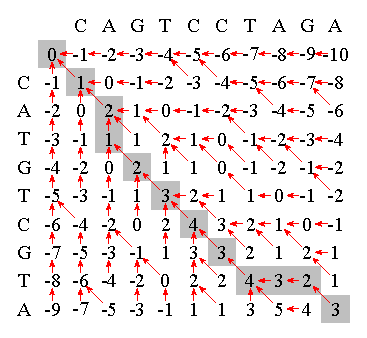
\includegraphics[width=\textwidth]{images/global_alignment}
    \end{subfigure}
    ~
    \begin{subfigure}[m]{0.3\textwidth}
    \centering
    \begin{verbatim}
    CATGTCAT--A
    CA-GTCCTAGA
    \end{verbatim}
    \end{subfigure}
    \caption[Globálne zarovnanie]{Globálne zarovnanie - vľavo je tabuľka dynamického programovania pre sekvencie vpravo}
    \label{fig:global-align}
\end{figure}

Algoritmus postupne vypĺňa 2-rozmernú maticu $A$. Riadky zodpovedajú bázam sekvencie $X$ a stĺpce bázam $Y$. Na políčku $A[i,j]$ bude skóre najlepšieho zarovnania prvých $i$ báz sekvencie $X$ a prvých $j$ báz $Y$.

Keď zarovnávame sekvenciu s prázdnou sekvenciou, tak skóre bude $-n$, kde $n$ je dĺžka sekvencie. Bude tam $n$ pomlčiek, každá nám dá skóre $-1$. Takto vyplníme riadky a stĺpce $A[i,0]$ a $A[0,j]$.

Ak chceme vyplniť políčko $A[i,j]$, musíme si uvedomiť ako môže vyzerať posledný stĺpec zarovnania $x_1x_2\dots x_i$ a $y_1y_2\dots y_j$. Máme iba 3 možnosti ako môže vyzerať posledný stĺpec najlepšieho zarovnania. Buď obsahuje $x_i$ alebo $y_j$ alebo oboje. V prípade, že posledný stĺpec obsahuje oboje, cena tohto stĺpca je buď $+1$ ak $x_i = y_j$ alebo $-1$ ináč. Ak by sme posledný stĺpec zmazali, dostali by sme zarovnanie $x_1x_2\dots x_{i-1}$ a $y_1y_2\dots y_{j-1}$, pričom musí ísť o najlepšie zarovnanie. To už máme vypočítané v políčku $A[i-1, j-1]$, čiže výsledné skóre bude $A[i-1, j-1] + s(x_i,y_j)$.

V prípade, že posledný stĺpec obsahuje len $x_i$ zarovnané s pomlčkou, skóre stĺpca bude $-1$ a po zmazaní dostávame zarovnanie $x_1x_2\dots x_{i-1}$ a $y_1y_2\dots y_{j}$, výsledné skóre bude teda $A[i-1, j] -1$. V prípade, že posledný stĺpec obsahuje len $y_i$, tak skóre vypočítame analogicky.

Najlepšie skóre bude maximálne skóre pre všetky 3 prípady.
Dostávame teda nasledujúci vzťah pre výpočet $A[i,j]$:
$$A[i,j] = \max \left\{
\begin{array}{l}
A[i-1,j-1]+s(x_i, y_j)\\
A[i-1,j]-d\\
A[i,j-1]-d
\end{array} \right.$$
Maticu vieme vypĺňať po riadkoch, pričom každé políčok vieme vypočítať z troch políčok, ktoré už sú vypočítané. Políčko $A[0, 0] = 0$ a krajné políčka potom vieme vypočítať ako $A[i,0] = A[i-1,j]-d$ a $A[0, j] = A[i,j-1]-d$

Ak nás zaujíma aj zarovnanie -- nie len jeho skóre -- vieme si pre každé políčko zapamätať ktorá z 3 možností dosiahla maximálnu hodnotu
(červené šípky na Obr. \ref{fig:global-align}). Na základe tejto informácie potom vieme zrekonštruovať zarovnanie tak, že postupne z posledného políčka ($A[n,m]$) budeme prechádzať na políčko, z ktorého sme vypočítali aktuálnu hodnotu.

Časová zložitosť je $O(nm)$, pretože vypĺňame $nm$ políčok, každé v konštantnom čase. Zjavne aj pamäťová zložitosť je $O(nm)$.

Pamäťová zložitosť sa dá zredukovať na $O(n+m)$ za cenu zhruba dvojnásobného času výpočtu \cite{hirschberg}.

\subsection{Algoritmus pre lokálne zarovnanie: Smith-Waterman}

% TODO: preformulovať aby sedelo na lokalne zarovnania
%Máme dané 2 sekvencie $X = x_1x_2\dots x_n$ a $Y = y_1y_2\dots y_n$, budeme zarovnávať všetky znaky sekvencie $X$ a všetky znaky sekvencie $Y$. Budeme používať jednoduché skórovanie: $+1$ za zhodu, $-1$ za nezhodu alebo pomlčku.

\begin{figure}[htp]
    \centering
    \begin{subfigure}[m]{0.5\textwidth}
    \centering
    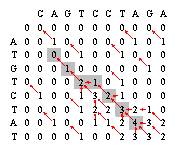
\includegraphics[width=\textwidth]{images/local_alignment}
    \end{subfigure}
    ~
    \begin{subfigure}[m]{0.3\textwidth}
    \centering
    \begin{verbatim}
    GT-CTA
    GTCCTA
    \end{verbatim}
    \end{subfigure}
    \caption[Lokálne zarovnanie]{Lokálne zarovnanie - vľavo je tabuľka dynamického programovania pre sekvencie vpravo}
    \label{fig:local-align}
\end{figure}

Algoritmus pre lokálne zarovnania sa líši len v niekoľkých malých detajloch. Opäť vypĺňame maticu $A$, s tým, že v $A[i,j]$ bude najvyššie skóre lokálneho zarovnania medzi sekvenciami $x_1x_2\dots x_i$ a $y_1y_2\dots y_j$, ktoré buď obsahuje bázy $x_i$ aj $y_j$, alebo je prázdne. Teda na ľubovoľnom mieste uvažujeme aj prázdne zarovnanie so skóre 0 (v matici nebudú záporné čísla). Vzťah pre výpočet $A[i,j]$ vyzerá takto:
$$A[i,j] = \max \left\{
\begin{array}{l}
0\\
A[i-1,j-1]+s(x_i, y_j)\\
A[i-1,j]-d\\
A[i,j-1]-d
\end{array} \right.$$
V tomto prípade sú všetky krajné políčka nulové.

Časová aj pamäťová zložitosť sú, rovnako ako pri globálnom zarovnaní $O(nm)$.

\subsection{Afínne skórovanie medzier}
\label{subsec:affine-gap-scoring}
V jednoduchom skórovaní sme dávali za pomčlku vždy rovnaké skóre ($-1$). Pri evolúcii sa však môže stať, že sa naraz zmaže niekoľko susedných báz. Pri \textit{afínnom skórovaní medzier} teda zavedieme dva typy skóre. Skóre za \textit{začatie medzery} a skóre za \textit{rozšírenie medzery}.

Algoritmus globálneho zarovnania vieme upraviť nasledovne: Namiesto matice $A$ teraz budeme mať 3 matice $M$, $I_x$, $I_y$ zodpovedajúce trom situáciám (Obr. \ref{fig:affine-space-situations}).

\begin{figure}[htp]
    \centering
    \begin{subfigure}[m]{0.3\textwidth}
    \centering
    \begin{BVerbatim}[commandchars=\\\{\}]
    ACTx\textsubscript{i}
    AGTy\textsubscript{j}
    \end{BVerbatim}
    \caption{Mutácia($M$)}
    \end{subfigure}
    ~
    \begin{subfigure}[m]{0.3\textwidth}
    \centering
    \begin{BVerbatim}[commandchars=\\\{\}]
    ACTTAx\textsubscript{i}
    AGTy\textsubscript{j}--
    \end{BVerbatim}
    \caption{Inzercia v X ($I_x$)}
    \end{subfigure}
    ~
    \begin{subfigure}[m]{0.3\textwidth}
    \centering
    \begin{BVerbatim}[commandchars=\\\{\}]
    ACTx\textsubscript{i}--
    AGTATy\textsubscript{j}
    \end{BVerbatim}
    \caption{Inzercia v Y ($I_y$)}
    \end{subfigure}
    \caption[Situácie pri afínnoom skórovaní]{Tri situácie pri afínnoom skórovaní medzier}
    \label{fig:affine-space-situations}
\end{figure}

Nech $M[i,j]$ je najlepšie skóre prvých $i$ báz zo sekvencie $X$ a prvých $j$ báz zo sekvencie $Y$, pričom $x_i$ je zarovnané k $y_j$, $I_x[i,j]$ je najlepšie skóre ak $x_i$ je zarovnané k medzere a $I_y[i,j]$ je najlepšie skóre ak $y_j$ je zarovnané k medzere.

Označme si $d$ penaltu za začatie medzery a $e$ penaltu za rozšírenie medzery. Vzťahy pre výpočet políčok sú nasledovné:
\begin{align*}
M[i,j] &= \max \left\{
\begin{array}{l}
M[i-1,j-1]+s(x_i, y_j)\\
I_x[i-1,j-1]+s(x_i, y_j)\\
I_y[i,j-1-1]+s(x_i, y_j)
\end{array} \right.\\
A[i,j] &= \max \left\{
\begin{array}{l}
M[i-1,j]-d\\
I_x[i-1,j]-e
\end{array} \right.\\
A[i,j] &= \max \left\{
\begin{array}{l}
M[i,j-1]-d\\
I_y[i,j-1]-e
\end{array} \right.
\end{align*}

V týchto rovniciach predpokladáme, že delécia nie je nasledovaná inzerciou. Toto platí v optimálnej sekvencii, ak $-d-s$ je menšie ako najmenšie skóre nezhody.

Tieto vzťahy vieme popísať stavovým diagramom na obrázku \ref{fig:alignment-fsa}:
\begin{figure}[h]
    \centering
    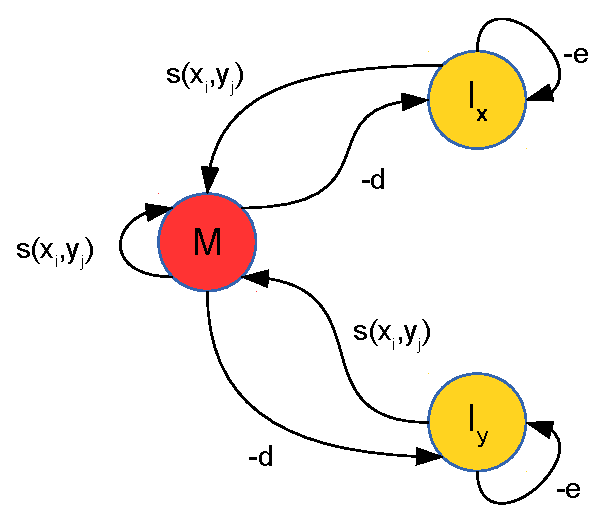
\includegraphics[width=.4\textwidth]{images/alignment_fsa}
    \caption[Stavový diagram pre zarovnanie sekvencií]{Stavový diagram pre zarovnanie sekvencií - obsahuje \textit{Match}~($M$), \textit{InsertX}~($I_x$) a \textit{InsertY}~($I_y$) stav a~prechody medzi nimi spolu s ich cenou. Napríklad prechod z $M$ do $I_x$ znamená vloženie medzery do $Y$-ovej sekvencie a to penalizujeme $-d$}
    \label{fig:alignment-fsa}
\end{figure}

Časová zložitosť je $O(nm)$, pretože vypĺňame $3nm$ políčok, každé v konštantnom čase. Pamäťová zložitosť je opäť $O(nm)$.

\cite{durbin}

\section[Zarovnávanie s HMM]{Zarovnávanie pomocou skrytých Markovových modelov}
\label{sec:hmm-alignment}

\subsection{Skryté Markovove modely (HMM)}
\textit{Skrytý Markovov model (hidden Markov model, HMM)} je pravdepodobnostý model, ktorý generuje náhodnú sekvenciu spolu s jej anotáciou (stavmi). HMM si móžme predstaviť ako konečný automat. Skladá sa z niekoľkých stavov, prechodov medzi nimi a emisií. Narozdiel od bežných konečných automatov, HMM emitujú symboly v stave, nie počas prechodu.
HMM sa skladá z 3 distribúcií
\begin{itemize}
\item distribúcia začiatočných stavov (HMM začne v stave $i$)
\item distribúcia prechodov (HMM prejde zo stavu $i$ do stavu $j$)
\item distribúcia emisií (HMM v stave $i$ vygeneruje symbol $x$)
\end{itemize}

Generovanie sekvencie teda vyzerá nasledovne: Na začiatku je HMM v niektorom stave (každý stav $i$ má nejakú pravdepodobnosť $\pi_i$, že bude začiatočný). Potom v každom kroku HMM emituje symbol $x$ s pravdepodobnosťou $e_{i, x}$ a prejde do stavu $j$ s pravdepodobnosťou $a_{i,j}$. Po $n$ krokoch takto vygenerujeme sekvenciu dľžky $n$, pričom každý symbol je oanotovaný stavom, ktorý ho vygeneroval.

V takomto modeli vieme počítať pravdepodobnosť, že model vygeneruje sekvenciu $x$ dĺžky $n$ s anotáciou $s$ ako súčin pravdepodobností prechodov a emisií.
Výpočet vyzerá nasledovne: $$P[X=x | S=s] = \pi_{s_1} e_{s_1,x1} a_{s_1,s_2} e_{s_2,x_2} a_{s_2,s_3} e_{s_3,x_3}\dots a_{s_{n-1},s_n} e_{s_n,x_n}$$.
\cite{skripta, durbin}

\subsection{Viterbiho algoritmus}
Hľadáme najpravdepodobnejšiu postupnosť stavov A, teda $\arg\max_A \Pr(A, S)$. Úlohu budeme riešiť dynamickým programovaním.

Podproblém $V[i,u]$ je pravdepodobnosť najpravdepodobnejšej cesty končiacej po $i$ krokoch v stave $u$, pričom vygeneruje $s_1 s_2 \dots s_i$.

\todo indexy su zle, napisat to trochu inac, asi cele do toho algoritmu, a mozno tie rekurentne vztahy zvlast nakoniec, alebo vynechat
\begin{subequations}
Rekurentné vzťahy pre náš algoritmus sú nasledovné:
\begin{align}
        \label{eq:viterbi-init}
        V[1,u] &= \pi_u e_{s_1, u}\\
        \label{eq:viterbi-step}
        V[i,u] &= \max_w V[i-1, w] a_{w,u} e_{s_i, u}
\end{align}
\end{subequations}

Algoritmus funguje takto:
Nech $n$ je dĺžka reťazca a $m$ je počet stavov.

\begin{lstlisting}[escapechar=\%]
%Nainicializuj $V[1,i]\, \forall i$ podľa \ref{eq:viterbi-init}%
for i in range(2, n):
    for u in range(1, m):
        %vypočítaj V[i, u] pomocou \ref{eq:viterbi-step}%
\end{lstlisting}
Maximálne V[n,j] je pravdepodobnosť najpravdepodobnejšej cesty
Aby sme vypísali anotáciu, pamätáme si pre každé V[i,u] stav w, ktorý viedol k maximálnej hodnote vo vzorci \ref{eq:viterbi-step}.

Časová zložitosť tohto algoritmu je $O(nm^2)$, kde $n$ je dľžka sekvencie a $m$ počet stavov.

Poznámka: pre dlhé sekvencie budú čísla V[i,u] veľmi malé a môže dôjsť k podtečeniu. V praxi teda používame zlogarimované hodnoty a namiesto násobenia súčet.

\subsection{Nastavenie parametrov HMM}
Ak máme oanotované trénovacie sekvencie, môžme z nich parametre odvodiť frekvenčnou analýzou. Emisie získame tak, že vyfiltrujeme symboly s príslušným stavom a spočítame frekvencie pre každý stav zvlášť a tranzície získame tak, že pre každý stav spočítame frekvencie nasledujúcich stavov. Tento postup sa volá \textit{metóda maximálnej vierohodnosti (v angličtine maximum likelihood estimation)}. \cite{ durbin, wiki:mle}

\subsection{Párové zarovnávanie pomocou HMM}
\todo mic odporúča rovno popísať párové hmm a aj viterbiho rovno naňom, takže to asi prepíšem

V časti \ref{subsec:affine-gap-scoring} sme si ukázali jednoduchý algoritmus na globálne zarovnávanie s afínnym skórovaním medzier. K tomuto algoritmu sme si uviedli aj jednoduchý stavový automat (Obr. \ref{fig:alignment-fsa}). Tento automat vieme previesť na HMM.

Na to aby sme automat previedli na HMM, musíme urobiť niekoľko zmien - musíme nastaviť emisné a tranzičné pravdepodobnosti, tak aby sumovali do jedna. Pre jednoduchosť pridáme aj prechody medzi stavmi $X a Y$. Ak ich pravdepodobnosti nastavíme na 0, máme model ekvivalentný predchádzajúcemu.

\begin{figure}[htp]
    \centering
    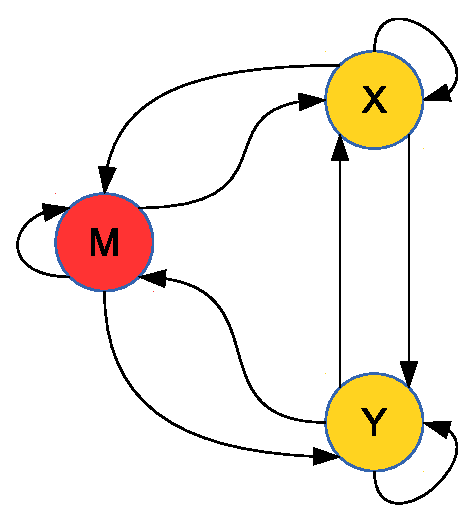
\includegraphics[width=.4\textwidth]{images/simple_model}
    \caption{Párový HMM pre zarovnávanie sekvencií}
    \label{fig:simple-model}
\end{figure}

Dostaneme model podobný HMM s tým rozdielom, že namiesto jedného symbolu emitujeme dvojicu symbolov. Takýto model sa nazýva \textit{Párový skrytý Markvov model}. Na tento model môžme použiť mierne modifikovaný Viterbiho algoritmus na nájdenie najpravdepodobnejšej postupnosti stavov, čo nám dá najpravdepodobnejšie zarovnanie.

Parametre modelu móžme ľahko natrénovať z existujúcich párových zarovnaní.

Nech dĺžky oboch sekvencií sú $O(n)$, a $m$ je počet stavov. Potom Viterbiho algoritmus na Párovom HMM bude bežať v čase $O(n^2m^2)$.
\cite{durbin}

\section[Štat. významnosť ]{Štatistická významnosť zarovnania}
Smith-Watermanov algoritmus nájde najlepšie lokálne zarovnanie, pre ľubovoľné dve sekvencie. Treba však rozhodnúť, či je zarovnanie dostatočne vierohodné na to, aby predstavovalo skutočnú podobnosť sekvencií a nie len najlepšie zarovnanie dvoch nesúvisiacich sekvencií.
Ako vodítko pri rozhodnutí sa používajú identifikátory \textit{štatistickej významnosti} zarovnania: \textit{P-hodnota (P-value)} alebo \textit{E-hodnota (E-value)}.

\begin{figure}[htp]
    \centering
    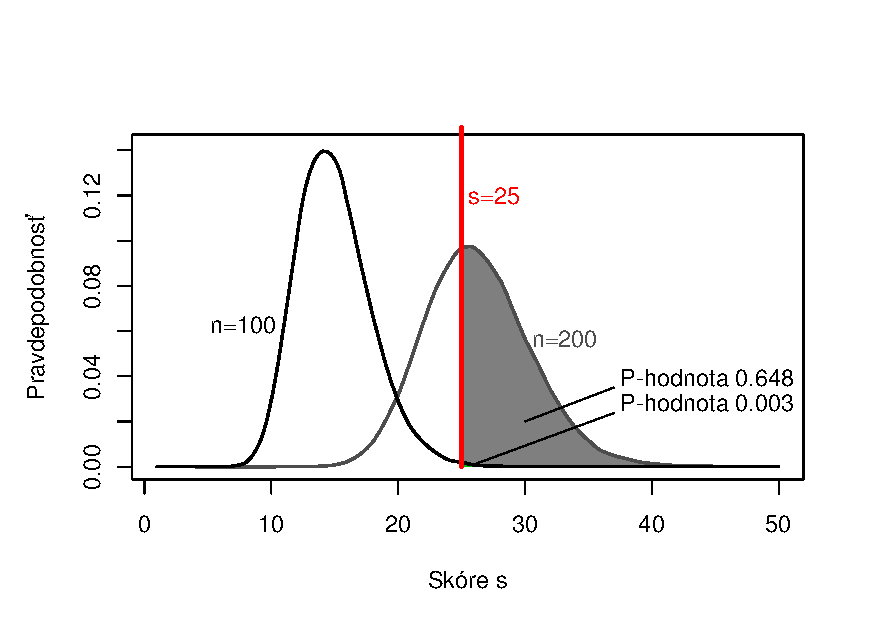
\includegraphics[width=.9\textwidth]{images/p-value}
    \caption[P-hodnota lokálneho zarovnania]{P-hodnota lokálneho zarovnania so skóre $s = 25$ medzi 2 sekvenciami dĺžky $n = 100$ alebo $n = 200$ (skórovanie $+1$ zhoda, $-1$ nezhoda alebo medzera). Rozdelenie bolo získané zarovnávaním $100000$ párov náhodných sekvencií. Pri $n=100$ je P-hodnota približne 0.003 a zodpovedá malej čiernej poloche pod krivkou napravo od zvislej čiary pre $s=25$. Pri dlhšich sekvenciách zodpovedá P-hodnota veľkej sivej ploche napravo od zvislej čiary. Pri takto dlhých sekvenciách očakáveme skóre 25 alebo väčšie vo viac ako 60\% prípadov čisto náhodou. Nejde teda o štatisticky významné zarovnanie.}
    \label{fig:p-value}
\end{figure}

P-hodnota zarovnania je pravdepodobnosť, že medzi nádhodne generovanými sekvenciami tej istej dĺžky by sme našli zarovnanie s rovnakým skóre alebo vyšším. Keďže P-hodnota závisí od dĺžok sekvencií a skóre, musíme ju počítať pri každom zarovnaní. Je však časovo náročné robiť to generovaním veľkého množstva zarovnaní, preto sa používajú matematicky odvodené vzorce na odhad tejto hodnoty. (\cite{Karlin}, \cite{Mitrophanov}).

E-hodnota vyjadruje strednú hodnotu počtu zarovnaní so skóre aspoň takým ako má naše zarovnanie medzi náhodne generovanými sekvenciami. E-hodnota teda môže byť aj väčšia ako jedna. Ak je E-hodnota väčšia ako jedna, tak čisto náhodou by sme očakávali aspoň 1 také silné zarovnanie a teda zarovnania s takouto (a nižšou) E-hodnotou nebudeme považovať za štatisticky významné.

V štatistike sa v rôznych testoch štandardne používajú prahy na P-hodnotu $0.05$ alebo $0.01$.
Pri zarovnávaní sekvencií však často používame ešte nižší prah, teda uvažujeme len zarovnania s P-hodnotou menšou ako napr. $10^{-5}$. Pri malých hodnotách sú P-hodnota a E-hodnota prebližne rovnaké, teda taký istý prah môžme použiť aj na E-hodnotu.
